%% content.tex
%%
\chapter{Choreoplethen-Karten}
\label{choreopleth}

\nocite{blocksmercator:2018}
\nocite{blockscolombia:2018}

\section{Allgemeines}
\label{sec:choreopleth-abstract}

Choreoplethenkarten unterscheiden sich von gewöhnlichen/einfachen Landkarten darin, dass bestimmte Abschnitte einer Karten einer bestimmten statistischen Variablen entsprechend eingefärbt werden. Daher rührt auch ihre alternative Bezeichnung als 'Thematische Karten'.

Nützlich ist diese Art einer Landkarte vor allem, um zu zeigen, wie Messungen/Werte in bestimmten geographischen Regionen variieren, sowie daraus gegebenenfalls Schlüsse zu ziehen. Ein Beispiel hierfür wäre die Anzahl erwerbsloser Personen in Relation zur Einwohnerzahl für jeden Landkreis in Deutschland.

\section{Implementierung in D3.js}
\label{sec:choreopleth-implementation}

\subsection{Problematik bzgl. bisherigem Ansatz}

Beim Versuch, eine solche Choreoplethenkarten in D3.js zu implementieren, tritt ein Problem mit der bisherigen Implementierung auf. Diese bildet zwar alle Länder ab, nutzt hierzu aber lediglich einen einzelnen Pfad, welcher folglich auch nur mit einer einzelnen Farbe gefüllt werden kann, was die Vergleichbarkeit von Regionen unmöglich macht.

Man muss also zunächst die Implementierung so abändern, dass statt einem Pfad für alle Länder ein Pfad pro Land gezeichnet wird. Möglich wird dies, wenn man statt dem übergebenen GeoJSON-Objekt als Ganzes nur das "features"-Array unter Zuhilfenahme des Enter-Update-Exit-Patterns an die Funktion übergibt.

\subsection{Implementierungsansatz zur Bewältigung}

Der allgemeine Teil und der Teil zum Anlegen von Projektions- und Pfadfunktion gestalten sich wie in \ref{sec:map-abstract} und \ref{sec:map-setup} beschrieben. Danach folgt das veränderte Einlesen der Datei wie folgt:

\begin{lstlisting}

var url = "...";

d3.json(url, function(geojson){
    svg.selectAll("path")
            .data(geojson.features)
            .enter()
            .append("path")
            .attr("d", path);
})

\end{lstlisting}

\subsection{Einfärbung der Landkarte}

Um nun noch gemäß der Aufgabenstellung jedes Land entsprechend seiner Kennzahl einfärben zu können, muss eine Farbskala erstellt werden. Beim Zeichnen der Pfade wird dann die jeweilige Füllfarbe mithilfe des Werts der entsprechenden Kennzahl und der Farbskala berechnet und gesetzt.

Der allgemeine Teil und der Teil zum Anlegen von Projektions- und Pfadfunktion gestalten sich erneut wie in \ref{sec:map-abstract} und \ref{sec:map-setup} beschrieben. Danach folgt das Einlesen der Datei und Einfärben der Pfade wie folgt (Kennzahl ist das Bruttoinlandsprodukt jeden Landes, das in der GeoJSON-Datei über den optionalen Wert "properties" mit übergeben wird)

\begin{lstlisting}

var url = "...";

d3.json(url, function(geojson){
    var features = geojson.features;

    var min = d3.min(features, function(d){
        return d.properties.gdp_md_est;
    });

    var max = d3.max(features, function(d){
        return d.properties.gdp_md_est;
    });

    var color = d3.scaleLinear()
            .domain([min, max])
            .range(["white", "crimson"]);

    svg.selectAll("path")
            .data(features)
            .enter()
            .append("path")
            .attr("d", path)
            .style("fill", function(d){
                return color(d.properties.gdp_md_est);
            });
});

\end{lstlisting}

Die entstehende Landkarte hat dieses Aussehen:

\begin{figure}[H]
    \centering
    
    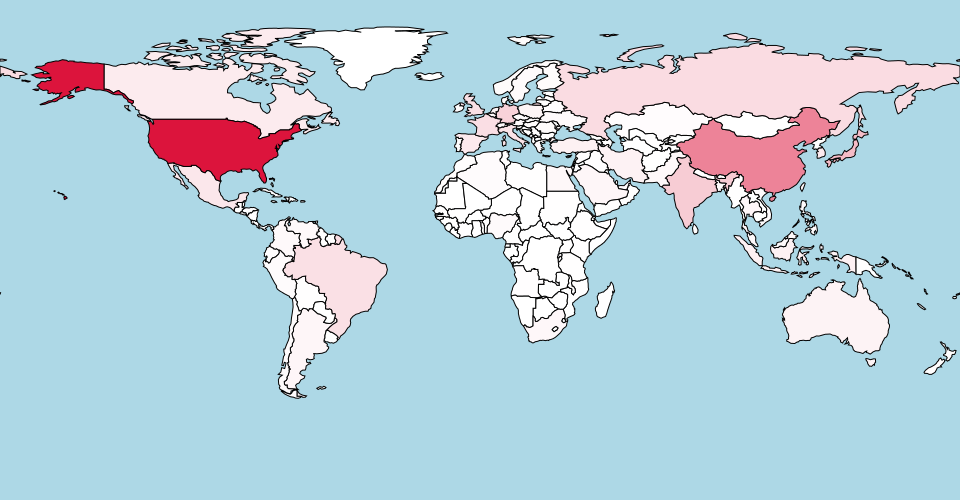
\includegraphics[width=.5\textwidth]{images/mapChoreopleth}
    \caption{\glqq Natural Earth\grqq -Projektion}
\end{figure}